\documentclass{article}
\usepackage{graphicx}
\usepackage{tabularx}
\usepackage{natbib}

\usepackage{array}
\usepackage{amsmath}
%\usepackage[backend=bibtex]{biblatex}
\bibliographystyle{..//refs/styles/besjournals.bst}
\setkeys{Gin}{width=0.8\textwidth}
%\setlength{\captionmargin}{30pt}
\setlength{\abovecaptionskip}{10pt}
\setlength{\belowcaptionskip}{10pt}
 \topmargin -1.5cm 
 \oddsidemargin -0.04cm 
 \evensidemargin -0.04cm 
 \textwidth 16.59cm
 \textheight 21.94cm 
 \parskip 6.2pt 
\renewcommand{\baselinestretch}{1.3} 
\AtBeginEnvironment{thebibliography}{\linespread{1}\selectfont}
\parindent 0pt
\renewcommand{\thetable}{S\arabic{table}}
\renewcommand{\thefigure}{S\arabic{figure}}
%\usepackage{xr}
%\usepackage{hyperref}
\usepackage{xr-hyper}
\usepackage{hyperref}
\externaldocument{invasive}
\title{Supporting Information: Seedling competition between a native %Honewort (\textit{Cryptotaenia canadensis}) 
and an invasive %Dame's Rocket (\textit{Hesperis matronalis}) 
woodland herb is mediated by relative germination timing}
\date{}
\usepackage{Sweave}
\begin{document}
\input{SUPPinvasive-concordance}


\maketitle
\section*{Tables}
%\begin{table}[hp]
%\centering
%\begin{tabular}{|l|l|l|}
%\hline
%species & seed source & status  \\
%\hline
%\textit{Anemone virginiana} & Prairie Moon & native  \\
%\textit{Asclepias syriaca} & Toadshade & native  \\
%\textit{Carex grayi} & Prairie Moon & native  \\
%\textit{Cryptotaenia canadensis} & Prairie Moon & native  \\
%\textit{Eurybia divaricata} & Toadshade & native  \\
%\textit{Hesperis matronalis} & American Meadows & invasive  \\
%\textit{Oenethera biennis} & Toadshade & native  \\
%\textit{Persicaria virginiana} & Prairie Moon & native  \\
%\textit{Silene stellata} & Prairie Moon & native  \\
%\textit{Silene vulgaris} & wild collected & invasive  \\
%\textit{Thalictrum diocicum} & Prairie Moon & native  \\
%\hline
%\end{tabular}
%\caption{Species information for germination assays. Seed were sourced from a) Prairie Moon Nursery, Winona, MN b) Toadshade Wildflower Farm, Frenchtown, NJ, c) American Meadows, Shelburne VT, or d) wild collected in unmanaged sections of the Arnold Arboretum, Boston MA. }
%\label{tab:specs}
%\end{table}
\begin{table}[hp]
\centering
\begin{tabular}{|rr|cc|ll|}
   \hline
     & & Max germination (\%) & &
   Mean germination days & \\ 
  \hline
  Strat. & Inc.  & C. canadensis & H. matronalis & C. canadensis & H. matronalis \\ 
  \hline
0 & H & 0.07 (0.1) & 0.78 (0) & 15.25 (0) & 3.11 (0.6) \\ 
  & L & 0 (0) & 0.75 (0.1) & --- & 4.59 (0.7) \\ 
   \hline
 2 & H & 0.03 (0) & 1 (0) & 9 (1) & 2.3 (0.1) \\ 
  & L & 0.2 (0.2) & 0.82 (0.1) & 10.25 (0.3) & 2.57 (0.5) \\ 
   \hline
 4 & H & 0.18 (0.1) & 0.97 (0) & 9.83 (3.6) & 2.49 (0.3) \\ 
 & L & 0.58 (0.3) & 0.82 (0.1) & 11.06 (1.1) & 3.5 (0.6) \\ 
    \hline
    5 & H & 0.08 (0.1) & 1 (0) & 8.44 (4.7) & 2.33 (0.4) \\ 
 & L & 0.85 (0.1) & 0.9 (0.1) & 7.67 (0.5) & 2.62 (0.6) \\ 
   \hline
   6 & H & 0.25 (0.2) & 0.98 (0) & 13.5 (6.9) & 1.91 (0.2) \\ 
  & L & 0.77 (0.1) & 0.97 (0.1) & 8.11 (0.4) & 2.14 (0.2) \\ 
    \hline
    7 & H & 0.6 (0) & 0.87 (0) & 5.81 (0.2) & 2 (0) \\ 
 & L & 0.97 (0.1) & 1 (0) & 6.29 (0.2) & 2.15 (0.2) \\ 
    \hline
    8 & H & 0.5 (0.1) & 1 (0) & 7.4 (0.3) & 2.06 (0.2) \\ 
 & L & 0.98 (0) & 0.95 (0) & 6.09 (0.4) & 1.94 (0.1) \\ 
      \hline
   9 & H & 0.6 (0.1) & 0.98 (0) & 5.22 (0.7 & 1.74 (0.1) \\ 
 & L & 1 (0) & 0.93 (0.1) & 6.04 (0.5) & 1.78 (0) \\ 
      \hline
   11 & H & 0.73 (0.2) & 0.98 (0) & 4.61 (0.2) & 1.86 (0.1) \\ 
 & L & 0.93 (0.1) & 0.93 (0.1) & 5.04 (0.3) & 2.11 (0.5) \\ 
      \hline
   13 & H & 0.77 (0.2) & 0.88 (0) & 4.14 (0.3) & 1.89 (0.9) \\ 
 & L & 1 (0) & 0.98 (0 & 4.16 (0.2) & 1.42 (0.3) \\ 
   \hline
\end{tabular}
\caption{Final germination percentages and mean germination time for focal species under all experimental treatment combination. Incubation levels (Inc. H/L) indicate mean temperature treatments of 20$^\circ$C or 15$^\circ$C respectively and stratifcation level (strat.) indicates the number of weeks of cold stratification at 4$^\circ$C.}
\label{tab:germcomps}
\end{table}

\begin{table}[hp]
\centering
\begin{tabular}{rrrrrrr}
  \hline
 & Estimate & Est.Error & Q2.5 & Q25 & Q75 & Q97.5 \\ 
  \hline
Intercept & 2.59 & 0.25 & 2.10 & 2.41 & 2.76 & 3.09 \\ 
  n\_Cc & -0.41 & 0.03 & -0.47 & -0.43 & -0.38 & -0.34 \\ 
  n\_Hm & 0.12 & 0.03 & 0.07 & 0.11 & 0.14 & 0.17 \\ 
  priority & 0.15 & 0.03 & 0.08 & 0.13 & 0.17 & 0.21 \\ 
   \hline
\end{tabular}
\caption{Effect size estimates from relative growth rate difference (RGRD) models with 50\% and 95\% uncertainty intervals}
\label{tab:RGRD}
\end{table}

\pagebreak
\section*{Figures}
%\begin{figure}[hp]
%    \centering
%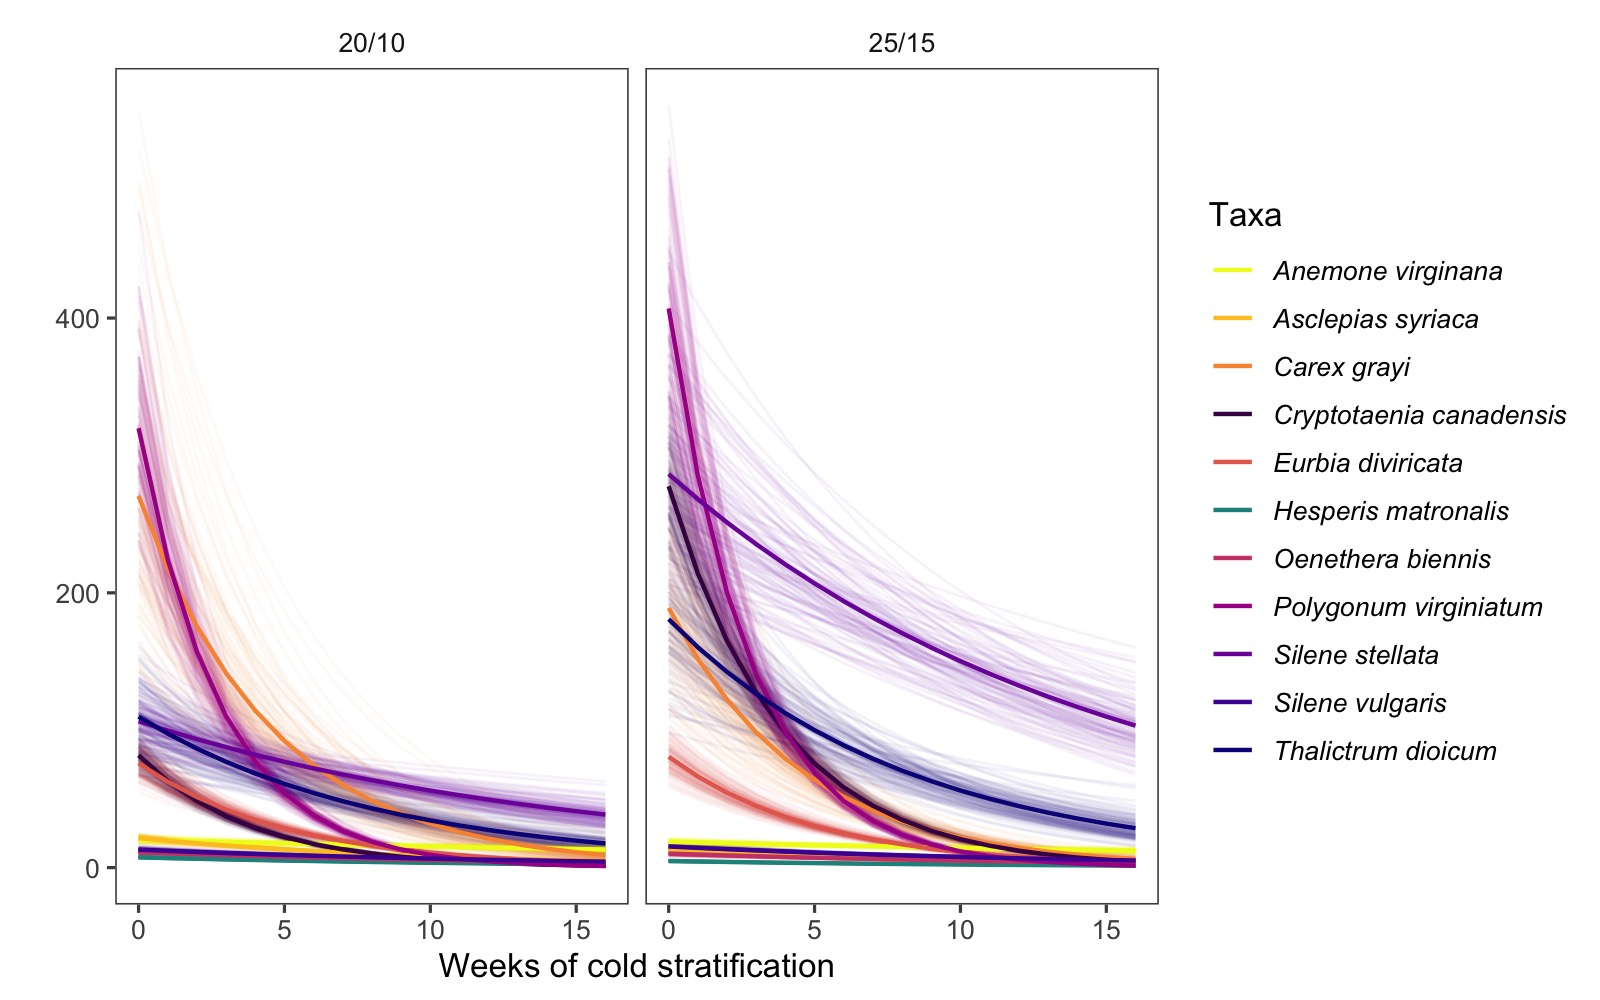
\includegraphics[width=\textwidth]{..//figure/AFTall.jpeg}
%   \caption{Estimated effect of weeks of cold stratification at 4$^\circ$C on the time to 50\% germination of 11 herbacious perennials under cool and warm (20/10$^\circ$C vs. 25/15$^\circ$C day/night) incubation conditions. The solid lines indicate the mean estimate, while lighter line indicate uncertainty.} 
%   \label{fig:AFTall}
%\end{figure}

\begin{figure}[hp]
    \centering
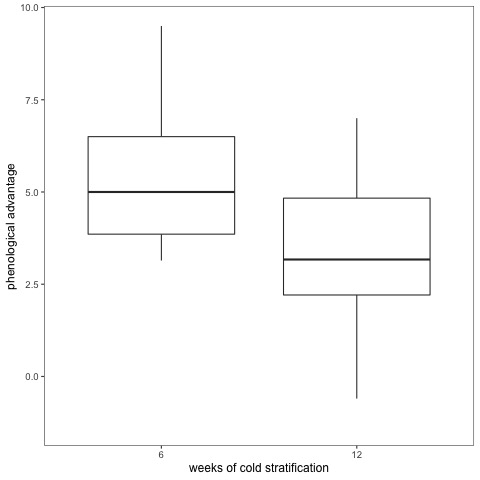
\includegraphics[width=.7\textwidth]{..//figure/priority_treat.jpeg}
   \caption{Differences in mean germination time (phenological advantage) between \textit{Hesperis matronalis} and \textit{Cryptotaenia canadensis} in each mixed-species pot under 6 and 12 weeks of cold stratification. Boxplots are based on raw data with middle bars indicating the median phenological advantage between the two species at each treatment level and the lower and upper hinges representing the 25\% and 75\% quantiles respectively} 
   \label{fig:MGTsup}
\end{figure}

\pagebreak
\section*{Measures of germination speed}
There are important differences between time to 50\% germination (t50) and mean germination time (MGT) that make one or the other more appropriate for the two types of experiments we ran. t50 is an estimate of the time to 50\% germination of all seeds planted, while mean germinating time (MGT) is a measure of the time to 50\% germination of only individuals that actually germinated \citep{Soltani:2015aa}. In comparative germination assays, t50 is considered a better metric because it standardizes phenological estimates across variable germination fractions. In our competition trials, we only wanted to estimate the phenology of individuals that germinated, so we used MGT as our measure of germination phenology. Because MGT is sensitive to the final germination fraction, it is not surprising the MGT measurements in the competition trials  were lower than the t50 estimates in the germination assays.

\bibliography{..///refs/germination.bib}

\end{document}
